\graphicspath{{Chapters/CrossSection/Figures/}}
\chapter{Observed Events and Cross Section Measurement}
\label{chap:CrossSection}

\section{Observed Events}

\begin{table}
\centering
\small
  \begin{tabular}{lcccc}
    \hline\hline
     7~\tev, \ZZ             & \eeee & \mmmm & \eemm & \llll \\
     \hline
Observed & 16 & 23 & 27 & 66 \\
Exp. Signal &   10.3 $\pm$ 0.1 $\pm$ 1.0 &  16.5 $\pm$ 0.2 $\pm$ 0.9 &  26.7 $\pm$ 0.2 $\pm$ 1.7 &  53.4 $\pm$ 0.3 $\pm$ 3.2 \\
Exp. Bg. & 0.5 $\pm$ 0.6 $\pm$ 0.3 & $<0.6$ & 0.7 $\pm$ 0.7 $\pm$ 0.6 & 0.9 $\pm$ 1.1 $\pm$ 0.7 \\
\hline\hline
    \\
    \hline\hline
     7~\tev, \ZZs             & \eeee & \mmmm & \eemm & \llll \\
     \hline
Observed & 21 & 30 & 33 & 84 \\
Exp. Signal &  12.3 $\pm$ 0.2 $\pm$ 1.2 &  20.5 $\pm$ 0.2 $\pm$ 1.1 &  31.6 $\pm$ 0.3 $\pm$ 2.0 &  64.4 $\pm$ 0.4 $\pm$ 4.0 \\
Exp. Bg. & 4.3 $\pm$ 1.4 $\pm$ 0.6 & $<0.9$ & 5.8 $\pm$ 1.6 $\pm$ 0.9 & 9.1 $\pm$ 2.3 $\pm$ 1.3 \\
    \hline\hline
  \end{tabular}

% $N_{Obs}$ \ZZ\ & 16 & 23 & 27 & 66 \\
% $N_{Obs}$ \ZZs\ & 21 & 30 & 33 & 84 \\
%      \hline
% $N^{Signal}_{Exp}$ \ZZ\ &   10.3 $\pm$ 0.1 $\pm$ 1.0 &  16.5 $\pm$ 0.2 $\pm$ 0.9 &  26.7 $\pm$ 0.2 $\pm$ 1.7 &  53.4 $\pm$ 0.3 $\pm$ 3.2 \\
% $N^{Signal}_{Exp}$ \ZZs\ &  12.3 $\pm$ 0.2 $\pm$ 1.2 &  20.5 $\pm$ 0.2 $\pm$ 1.1 &  31.6 $\pm$ 0.3 $\pm$ 2.0 &  64.4 $\pm$ 0.4 $\pm$ 4.0 \\
% \hline
% $N^{BG}_{Exp}$ \ZZ\   & 0.5 $\pm$ 0.6 $\pm$ 0.3 & $<0.6$ & 0.7 $\pm$ 0.7 $\pm$ 0.6 & 0.9 $\pm$ 1.1 $\pm$ 0.7 \\
% $N^{BG}_{Exp}$ \ZZs\ & 4.3 $\pm$ 1.4 $\pm$ 0.6 & $<0.9$ & 5.8 $\pm$ 1.6 $\pm$ 0.9 & 9.1 $\pm$ 2.3 $\pm$ 1.3 \\

  \caption{\label{tab:selected_data_MC}
           Summary of observed \ZZllll and \ZZsllll\ candidates in the data, total background estimates and expected signal
       for the individual decay modes (columns 2 to 4) and for their combination (last column).
       The quoted uncertainties and limits represent 68\% confidence intervals; the first uncertainty is statistical
           while the second is systematic. The uncertainty on the
       integrated luminosity (3.9\%) % and the theoretical uncertainties on the \ZZ cross section 
       is not included. %Contributions from a Higgs boson are not included in
       %the expected signal. 
          }
\end{table}

% 2D plot, 7 TeV
 \begin{figure}[htbp]
 \begin{center}
  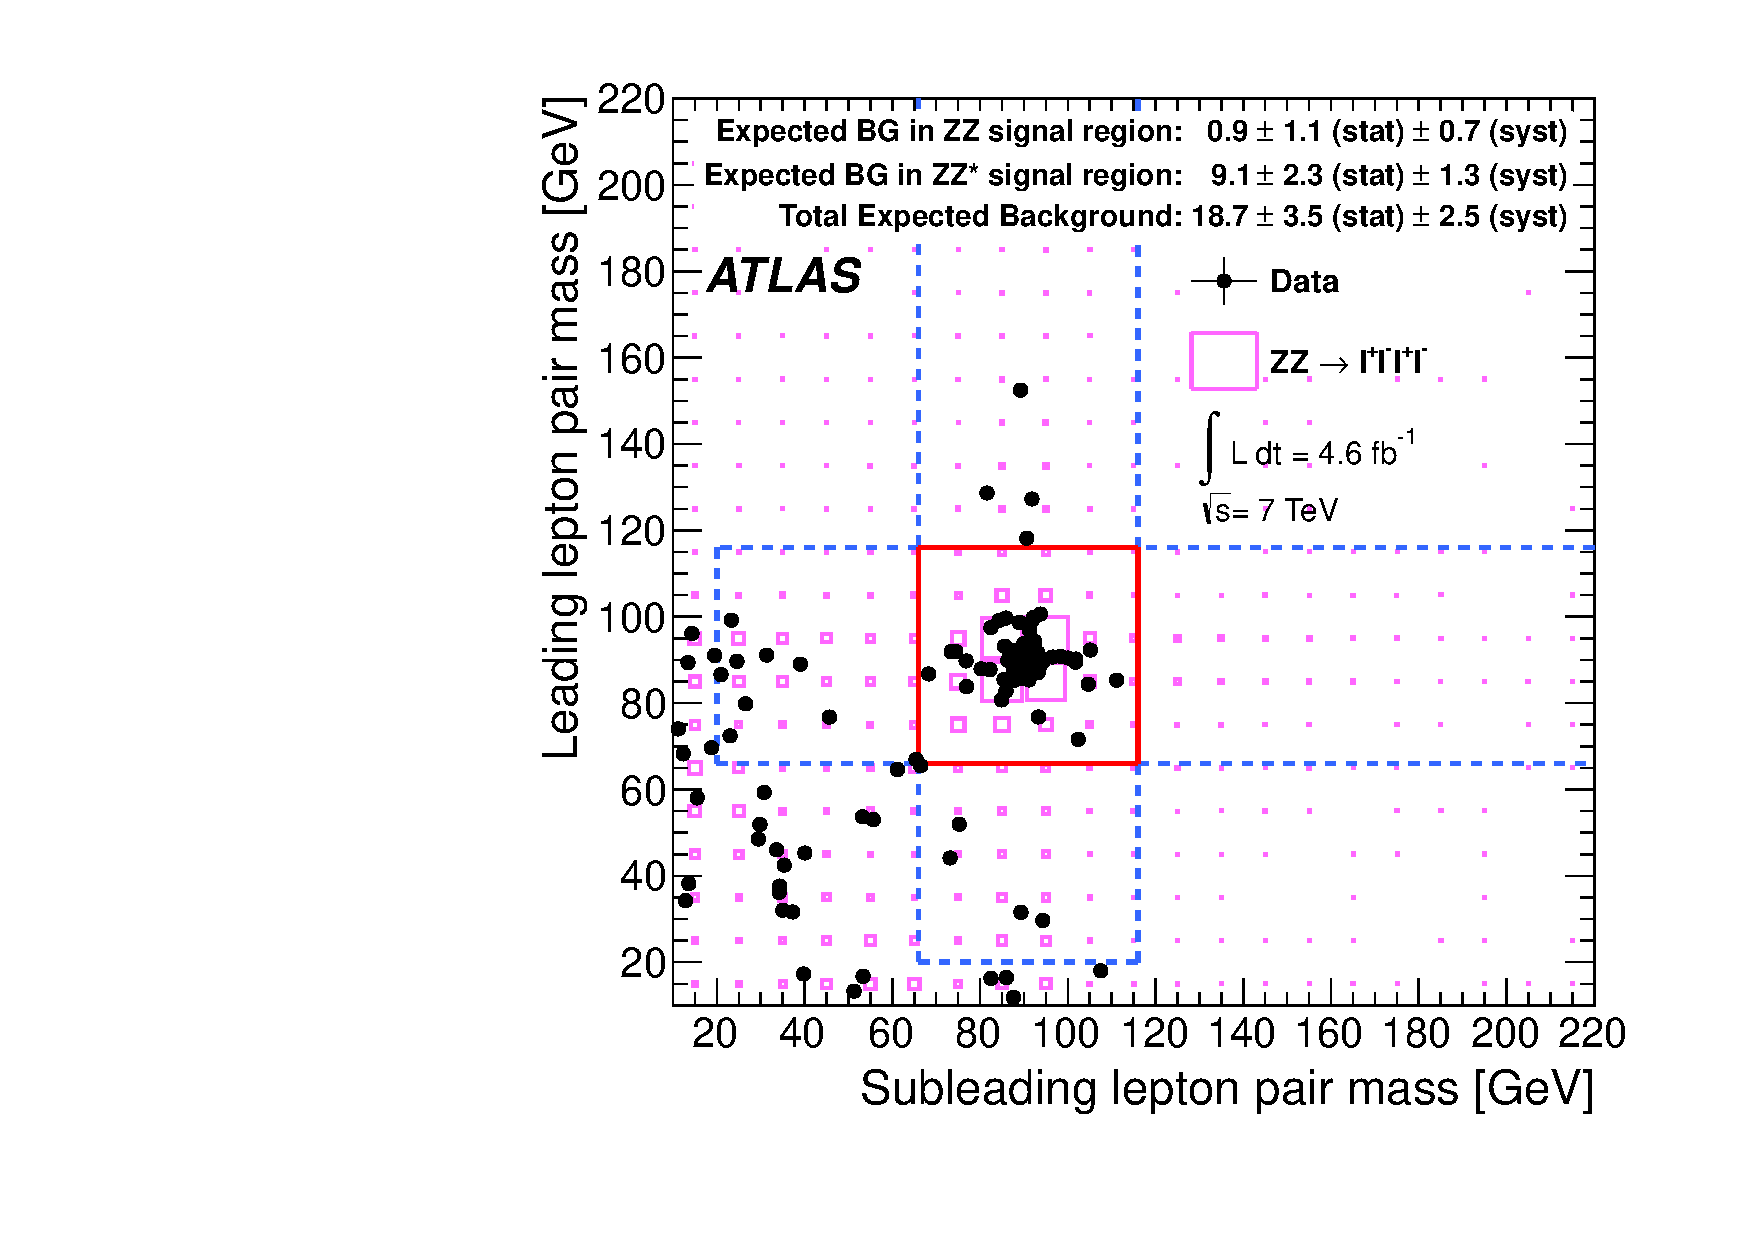
\includegraphics[width=0.7\textwidth]{7TeV/h_mz1_mz2}\hfill
  \caption[Mass of the leading \dilepton\ pair versus the mass of the
  sub-leading \dilepton\ pair for candidate events, passing all of the selection
  requirements apart from the \dilepton\ mass requirements, in the 7~\tev\ data.]
  {Mass of the leading \dilepton\ pair versus the mass of the
  sub-leading \dilepton\ pair for candidate events in the 7~\tev\ data after
  applying all of the selection
  requirements apart from the \dilepton\ mass requirements.
  The events observed in the data are shown as solid circles and the \ZZsllll\ signal prediction from simulation as boxes.
  The size of each box is proportional to the number of events in each bin.  
  The region enclosed by the solid (dashed) lines indicates the signal region defined by the
  \dilepton\ mass requirements on for \ZZ\ (\ZZs) events.
  %The background estimate is described in section 5.1.
   }
 \label{fig:mass2d}
 \end{center}
 \end{figure}

% pT_Z vs dR 7 TeV
% m_ZZ vs min(dR) 7 TeV

\subsection{Kinematic Distributions}

% 7 TeV, Z1_m, Z2_m, m_Z>7GeV
\begin{figure}[htbp]
    \begin{center}
     \subfigure[]{
     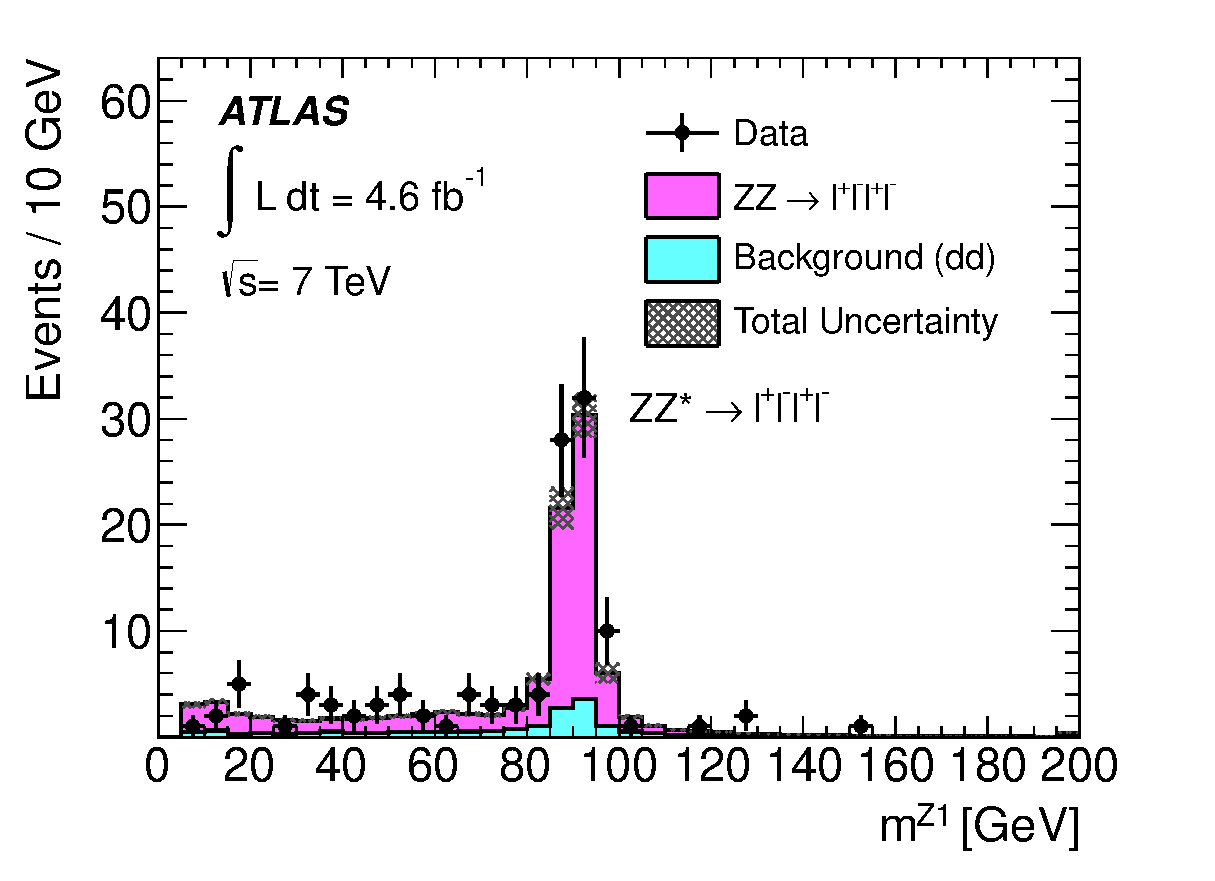
\includegraphics[width=0.47\textwidth]{7TeV/h_4l_ZZs_Z1_m}
     }
     \subfigure[]{
     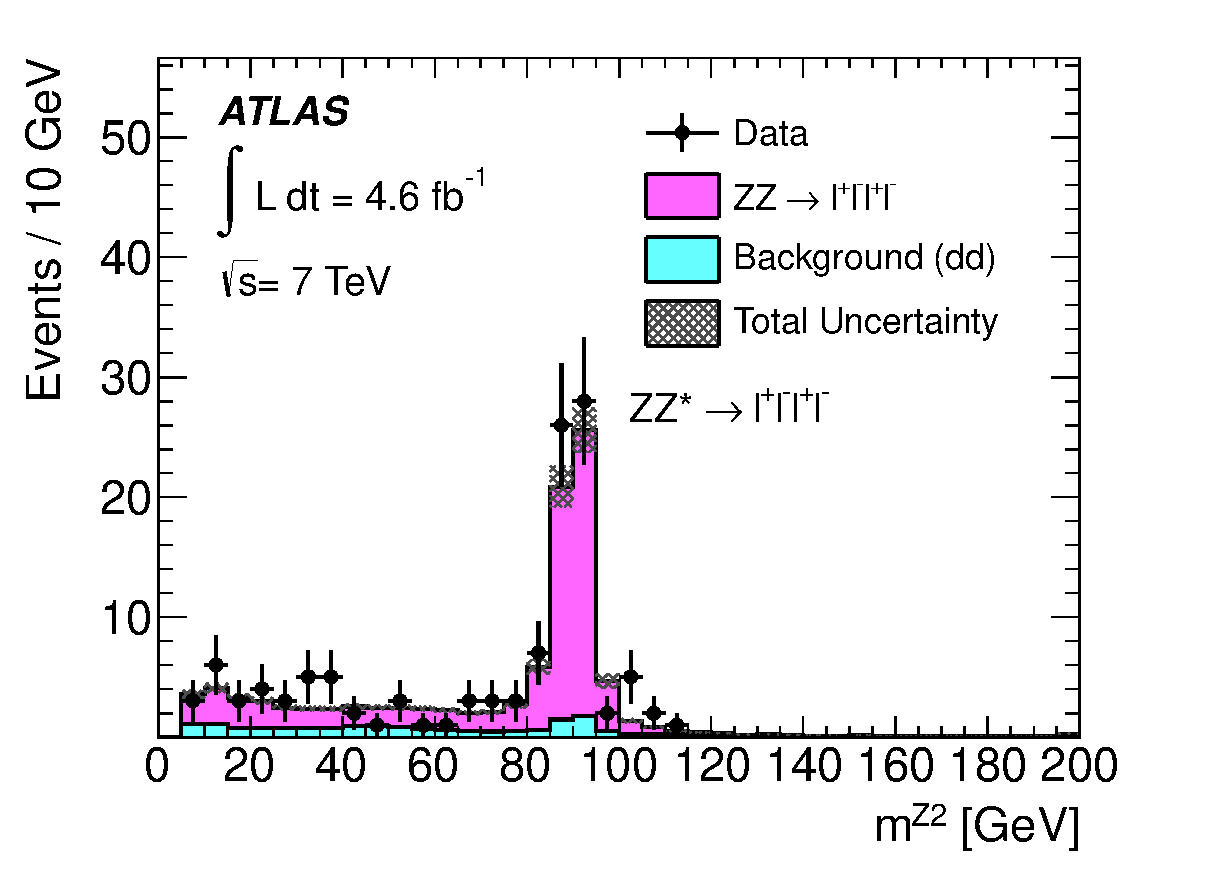
\includegraphics[width=0.47\textwidth]{7TeV/h_4l_ZZs_Z2_m}
     }
    \label{fig:zzdists-7tev-Zmass}
    \caption[Invariant masses of the (a) leading and (b) subleading \dilepton\ pair
    in candidate \ZZ\ events in the 7~\tev\ data.]
    {Invariant masses of the (a) leading and (b) subleading \dilepton\ pair
    in candidate \ZZ\ events in the 7~\tev\ data. Both \dilepton\ pairs are required to have
    $m_{\ell\ell}>7$~\gev.  The points represent the observed data and the
    histograms show the prediction from simulation, where the background is
    normalized to the data-driven estimate as described in
    ~\chap{BackgroundEsitmate}. The shaded band shows the combined statistical and
    systematic uncertainty on the prediction. 
}
\end{center}
\end{figure}

% 7 TeV, ZZ, ZZ_pt / ZZ_m
\begin{figure}[htbp]
    \begin{center}
     \subfigure[]{
     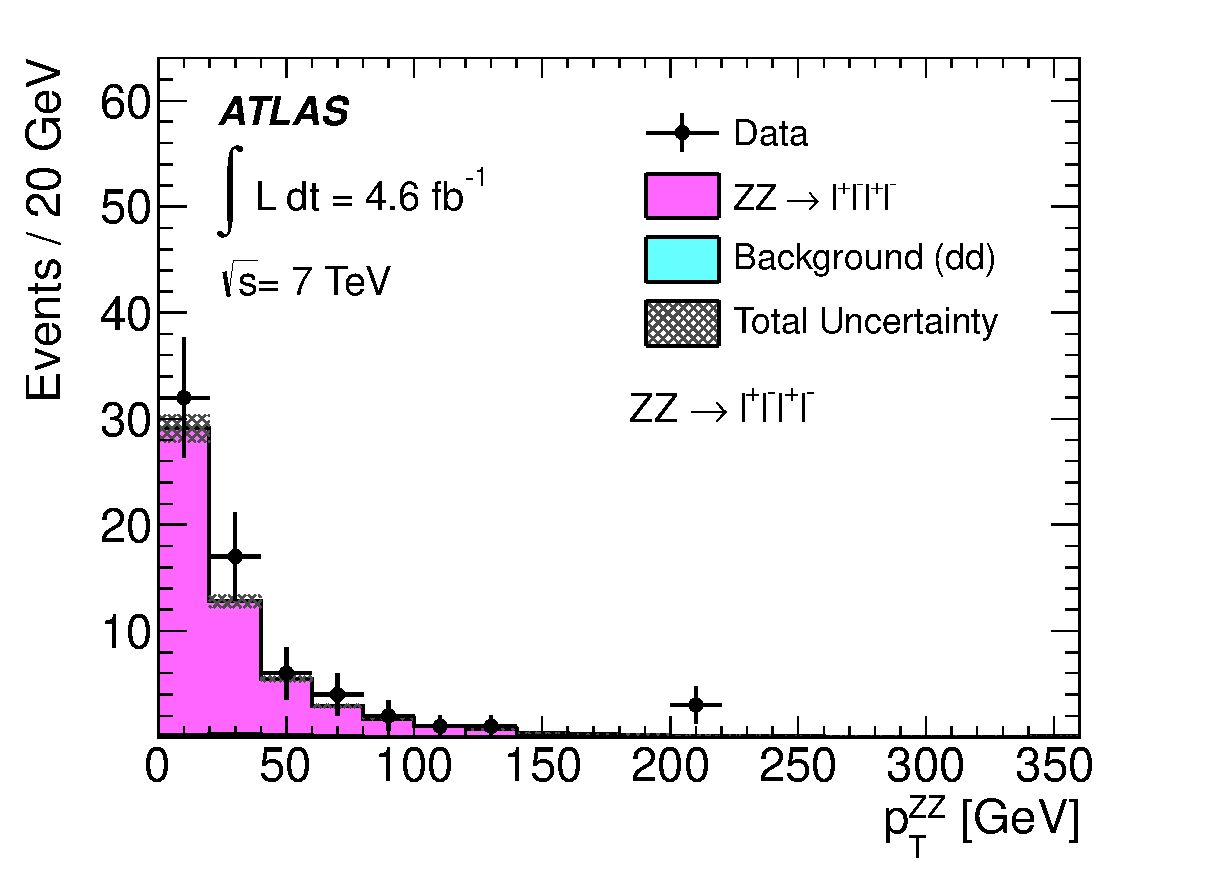
\includegraphics[width=0.47\textwidth]{7TeV/h_4l_ZZ_ZZ_pt}
     }
     \subfigure[]{
     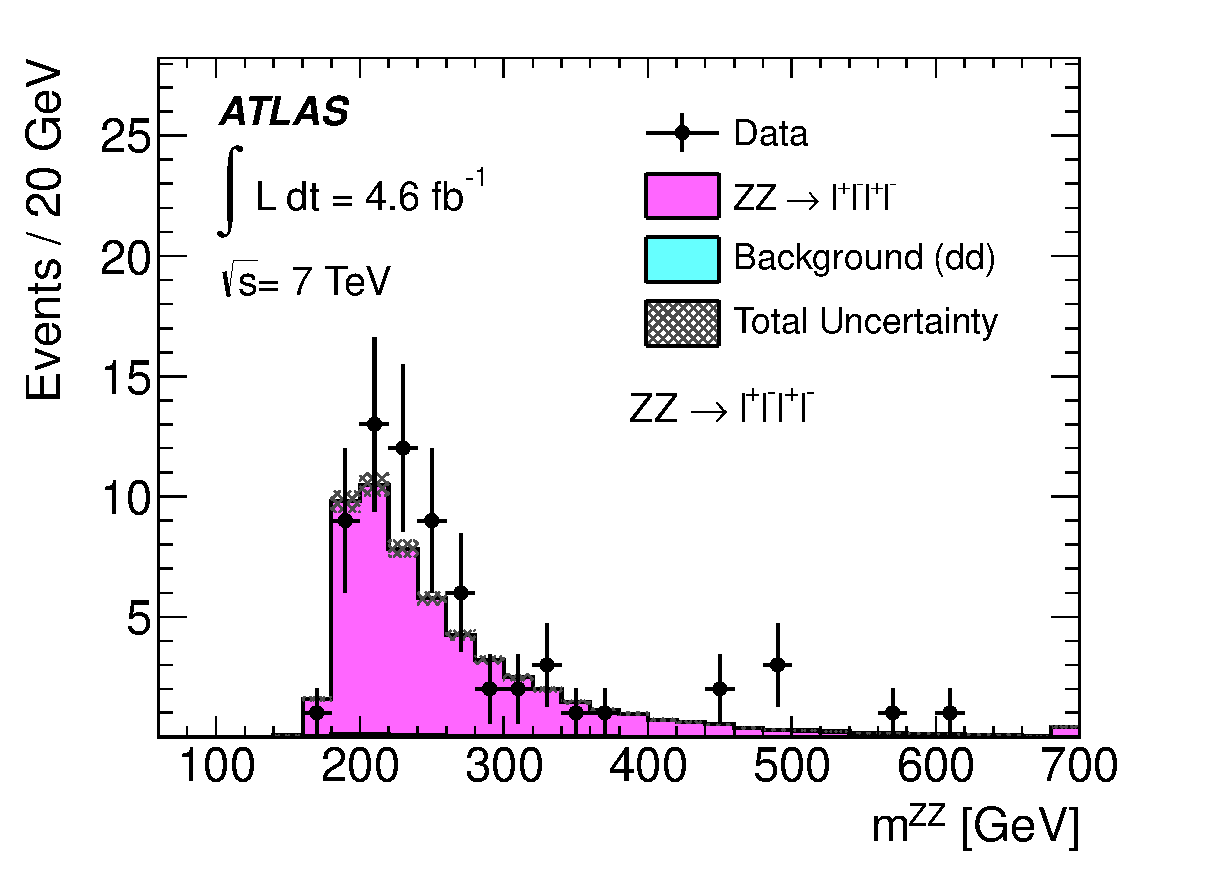
\includegraphics[width=0.47\textwidth]{7TeV/h_4l_ZZ_ZZ_m}
     }
     \subfigure[]{
     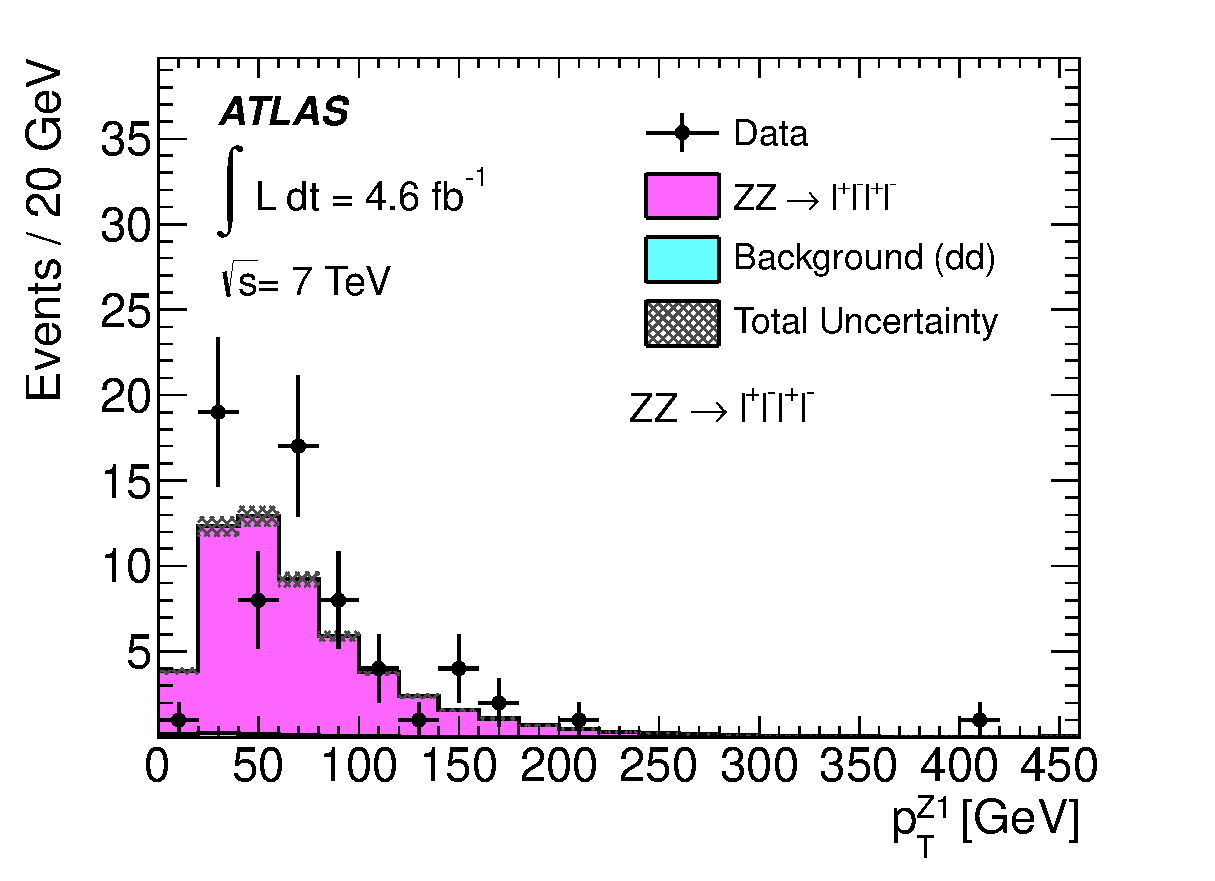
\includegraphics[width=0.47\textwidth]{7TeV/h_4l_ZZ_Z1_pt}
     }
     \subfigure[]{
     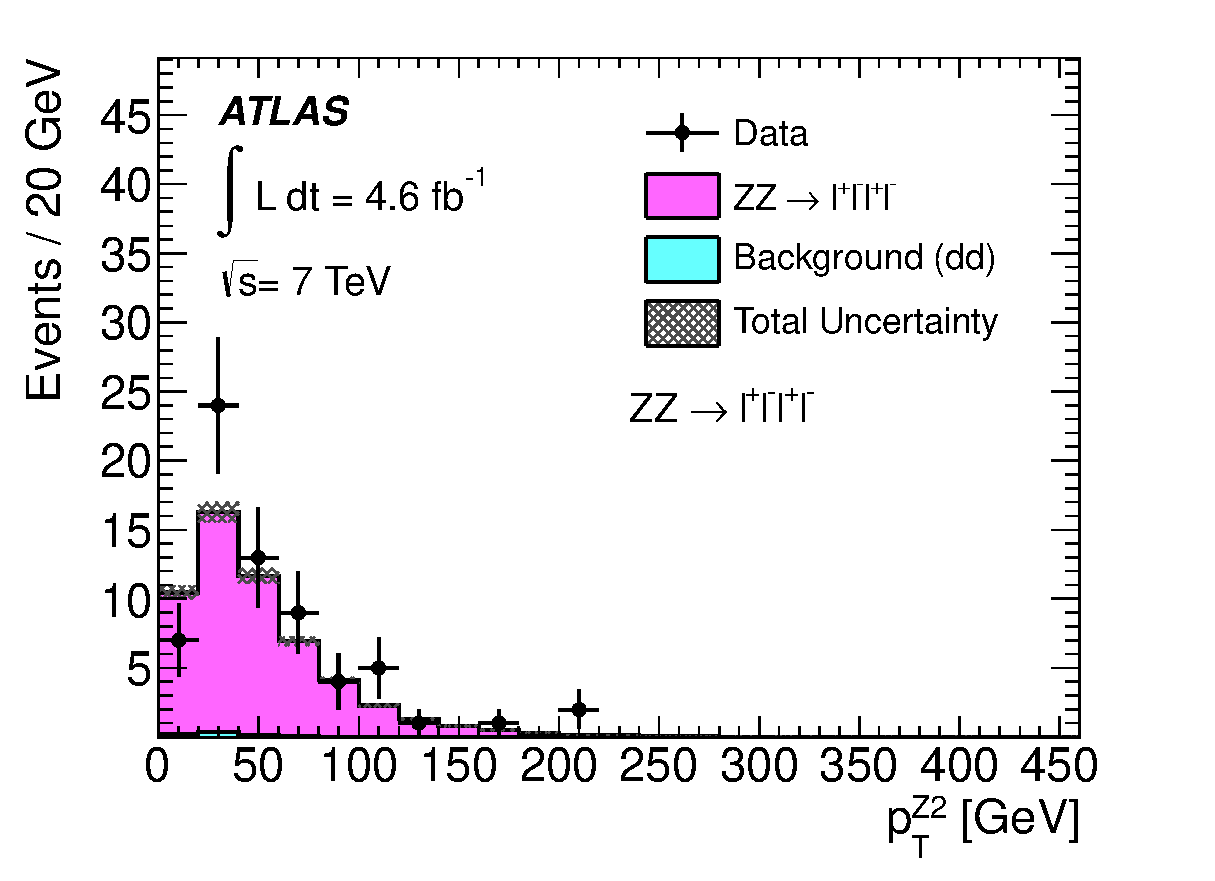
\includegraphics[width=0.47\textwidth]{7TeV/h_4l_ZZ_Z2_pt}
     }
    \label{fig:zzdists-7tev-ZZ}
    \caption[Kinematic distributions for events passing the \ZZ\ selection in
    the 7~\tev\ data.]
    {Kinematic distributions for events passing the \ZZ\ selection in
    the 7~\tev\ data: (a) transverse momentum $\pT^{\ZZ}$ and (b) invariant mass $m^{\ZZ}$ of the 
    four-lepton system, (c) transverse momentum of the leading
    dilepton pair $\pt^{Z1}$, and (d) transverse momentum of the subleading
    dilepton pair $\pt^{Z2}$. The points represent the observed data and the 
    histograms show the prediction from simulation, where the background
    is normalized to the data-driven (dd) estimate as described in ~\chap{BackgroundEsitmate}. The shaded band 
    shows the combined statistical and systematic uncertainty on the prediction. 
    }
    \end{center}
\end{figure}

% 7 TeV, ZZ*, ZZ_pt / ZZ_m
\begin{figure}[htbp]
\begin{center}
    \subfigure[]{
    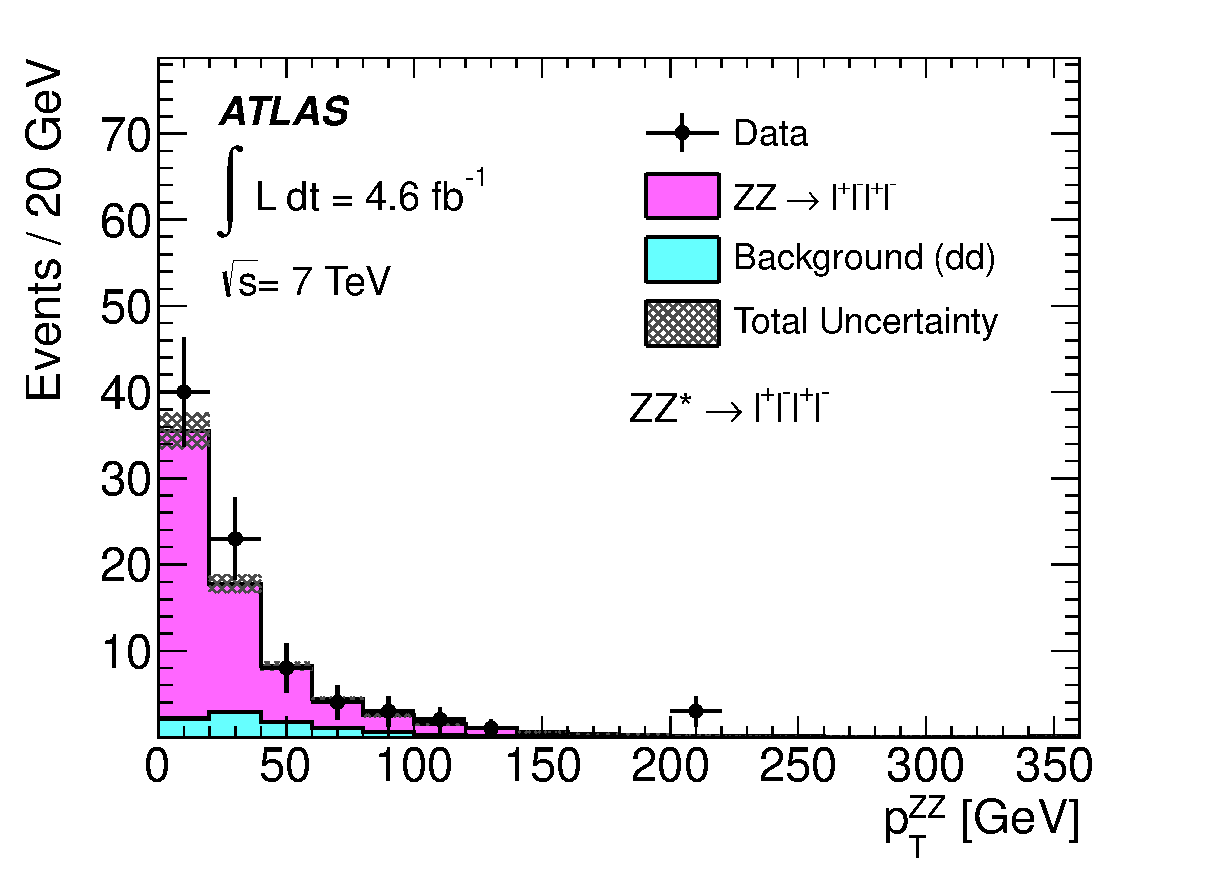
\includegraphics[width=0.47\textwidth]{7TeV/h_4l_ZZs_ZZ_pt}
    }
    \subfigure[]{
    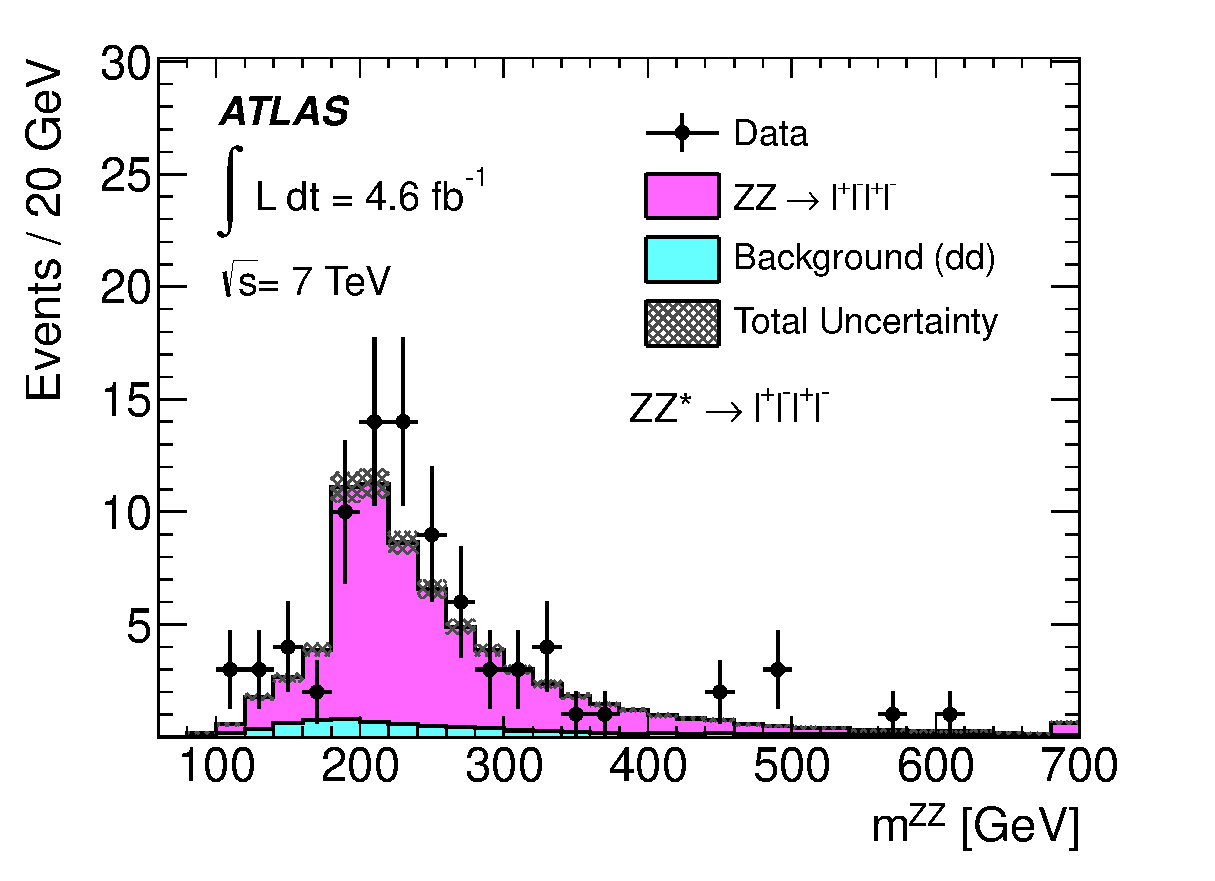
\includegraphics[width=0.47\textwidth]{7TeV/h_4l_ZZs_ZZ_m}
    }
    \subfigure[]{
    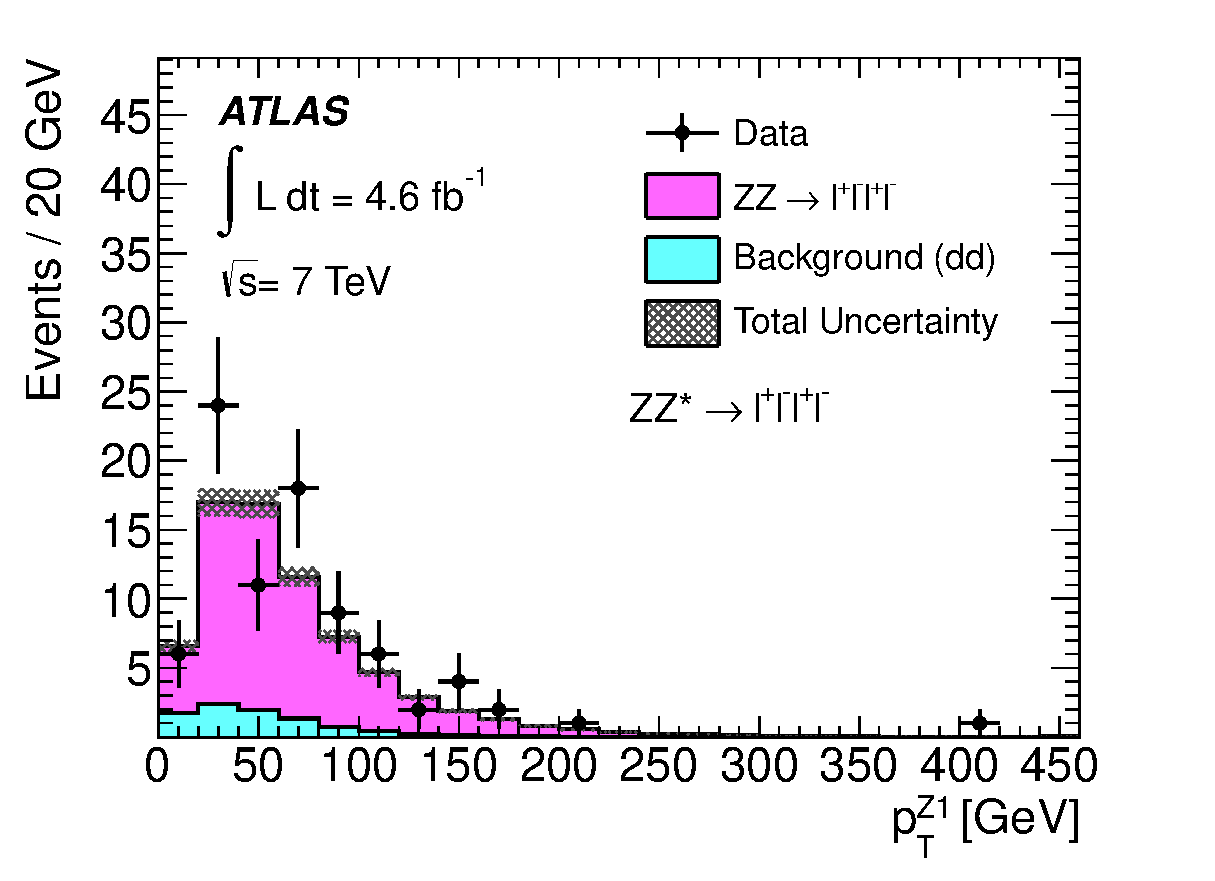
\includegraphics[width=0.47\textwidth]{7TeV/h_4l_ZZs_Z1_pt}
    }
    \subfigure[]{
    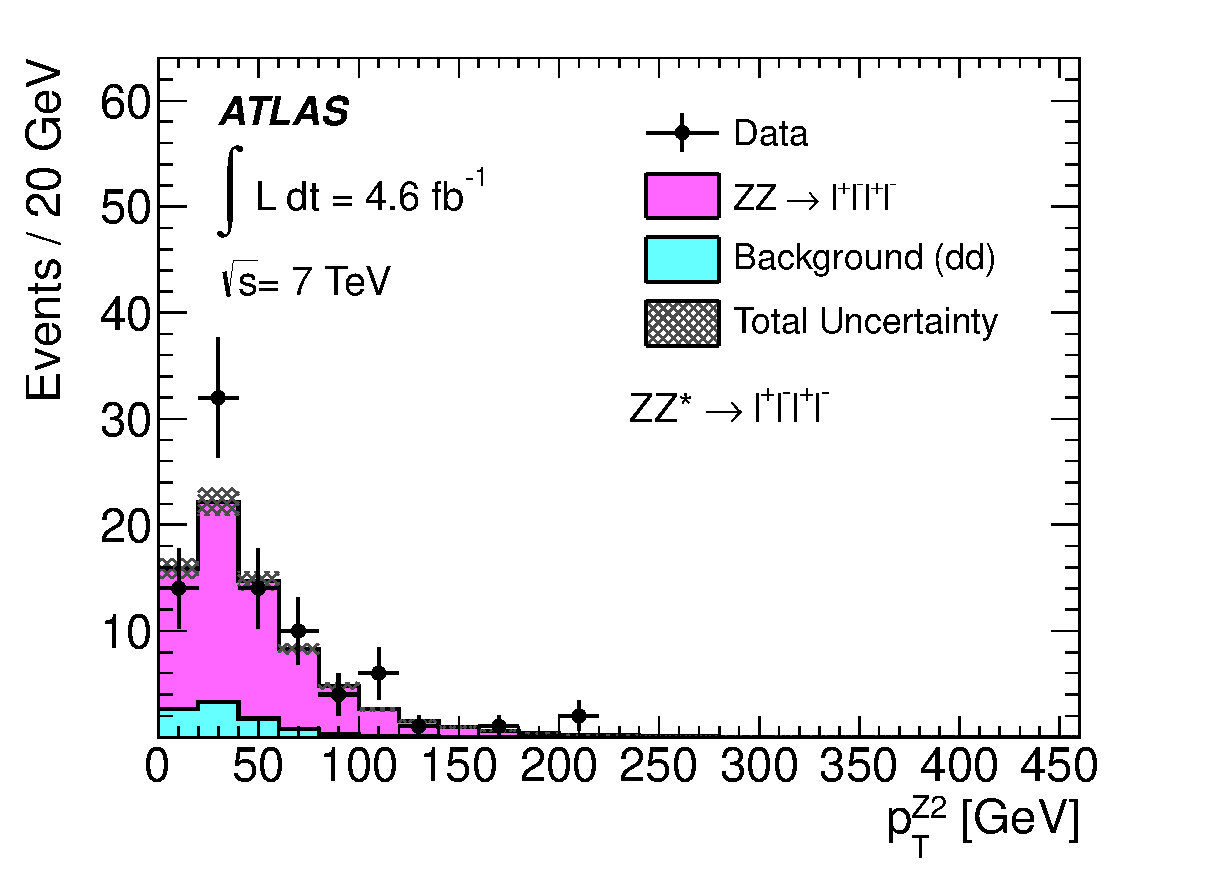
\includegraphics[width=0.47\textwidth]{7TeV/h_4l_ZZs_Z2_pt}
    }
    \label{fig:zzdists-7tev-ZZs}
    \caption[Kinematic distributions for events passing the \ZZs\ selection in
    the 7~\tev\ data.]
    {Kinematic distributions for events passing the \ZZs\ selection in
    the 7~\tev\ data: (a) transverse momentum $\pT^{\ZZ}$ and (b) invariant mass $m^{\ZZ}$ of the 
    four-lepton system, (c) transverse momentum of the leading
    dilepton pair $\pt^{Z1}$, and (d) transverse momentum of the subleading
    dilepton pair $\pt^{Z2}$. The points represent the observed data and the 
    histograms show the prediction from simulation, where the background
    is normalized to the data-driven (dd) estimate as described in ~\chap{BackgroundEsitmate}. The shaded band 
    shows the combined statistical and systematic uncertainty on the prediction. 
    }
\end{center}
\end{figure}

\section{Cross Section Measurement}
\subsection{Cross Section Definition}
\subsection{Fiducial Acceptance}
\subsection{Cross Section Extraction}
